% Fig. 3 -- DeXposure-Bench block diagram (TikZ, TKDE classic style)
% Drop-in replacement for figures/fig3_evaluation_framework.{pdf,png}.
%
% Required packages (already in main DeXposure-Agent.tex):
%   \usepackage{tikz}
%
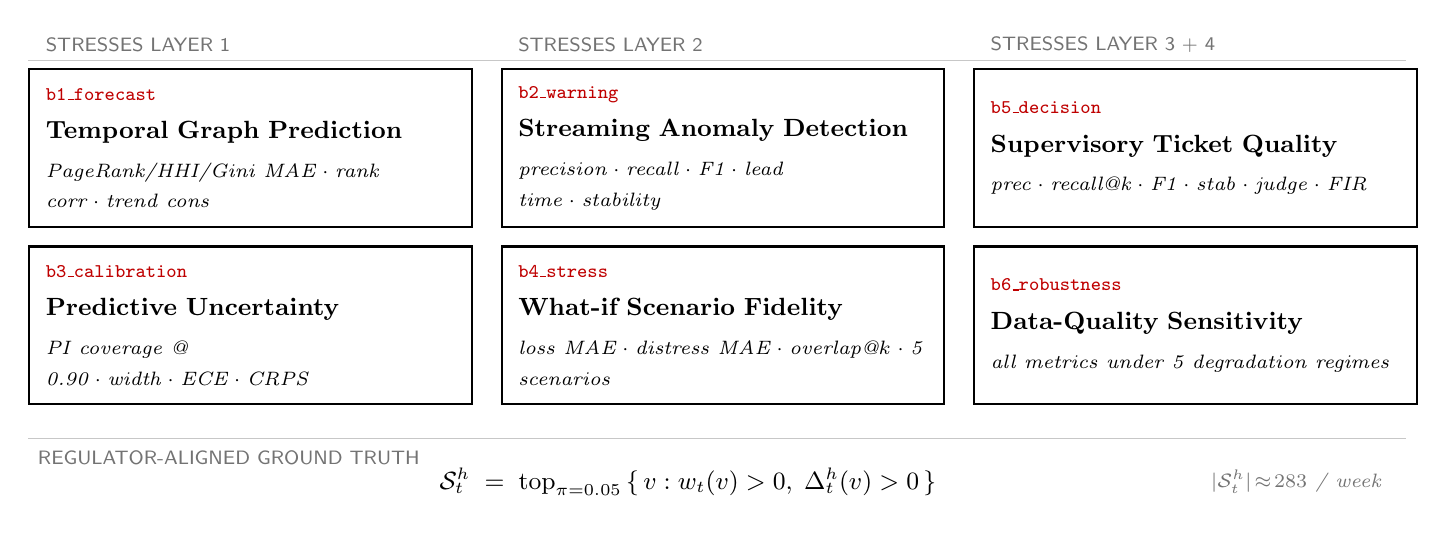
\begin{tikzpicture}[
  font=\small,
  card/.style     = {draw, thick, rectangle, minimum width=5.5cm, minimum height=2.0cm,
                     align=left, inner sep=6pt, text width=5.2cm},
  cardw/.style    = {draw, thick, rectangle, minimum width=5.8cm, minimum height=2.0cm,
                     align=left, inner sep=6pt, text width=5.5cm},
  tag/.style      = {font=\scriptsize\sffamily, text=black!55},
  bid/.style      = {font=\scriptsize\ttfamily\bfseries, text=red!75!black},
  rule/.style     = {draw=black!22, line width=0.35pt},
  hint/.style     = {font=\scriptsize\itshape, text=black!55},
]

% --- group headers (small caps row at top) ------------------------------
\node[tag, anchor=west] (h1) at (0,0.6) {STRESSES LAYER 1};
\node[tag, anchor=west] (h2) at (6.0,0.6) {STRESSES LAYER 2};
\node[tag, anchor=west] (h3) at (12.0,0.6) {STRESSES LAYER 3 + 4};

\draw[rule] (-0.1,0.4) -- (17.4,0.4);

% --- row 1 --------------------------------------------------------------
\node[card, anchor=north west] (b1) at (-0.1,0.3) {%
  {\scriptsize\ttfamily\bfseries\color{red!75!black} b1\_forecast} \\[3pt]
  \textbf{Temporal Graph Prediction} \\[3pt]
  \textit{\scriptsize PageRank/HHI/Gini MAE\;$\cdot$\;rank corr\;$\cdot$\;trend cons}
};

\node[card, anchor=north west] (b2) at (5.9,0.3) {%
  {\scriptsize\ttfamily\bfseries\color{red!75!black} b2\_warning} \\[3pt]
  \textbf{Streaming Anomaly Detection} \\[3pt]
  \textit{\scriptsize precision\;$\cdot$\;recall\;$\cdot$\;F1\;$\cdot$\;lead time\;$\cdot$\;stability}
};

\node[card, anchor=north west] (b5) at (11.9,0.3) {%
  {\scriptsize\ttfamily\bfseries\color{red!75!black} b5\_decision} \\[3pt]
  \textbf{Supervisory Ticket Quality} \\[3pt]
  \textit{\scriptsize prec\;$\cdot$\;recall@k\;$\cdot$\;F1\;$\cdot$\;stab\;$\cdot$\;judge\;$\cdot$\;FIR}
};

% --- row 2 --------------------------------------------------------------
\node[card, anchor=north west] (b3) at (-0.1,-1.95) {%
  {\scriptsize\ttfamily\bfseries\color{red!75!black} b3\_calibration} \\[3pt]
  \textbf{Predictive Uncertainty} \\[3pt]
  \textit{\scriptsize PI coverage @ 0.90\;$\cdot$\;width\;$\cdot$\;ECE\;$\cdot$\;CRPS}
};

\node[card, anchor=north west] (b4) at (5.9,-1.95) {%
  {\scriptsize\ttfamily\bfseries\color{red!75!black} b4\_stress} \\[3pt]
  \textbf{What-if Scenario Fidelity} \\[3pt]
  \textit{\scriptsize loss MAE\;$\cdot$\;distress MAE\;$\cdot$\;overlap@$k$\;$\cdot$\;5 scenarios}
};

\node[card, anchor=north west] (b6) at (11.9,-1.95) {%
  {\scriptsize\ttfamily\bfseries\color{red!75!black} b6\_robustness} \\[3pt]
  \textbf{Data-Quality Sensitivity} \\[3pt]
  \textit{\scriptsize all metrics under 5 degradation regimes}
};

% --- ground truth strip at bottom --------------------------------------
\draw[rule] (-0.1,-4.4) -- (17.4,-4.4);
\node[tag, anchor=west] at (-0.1,-4.65) {REGULATOR-ALIGNED GROUND TRUTH};

\node[anchor=west] at (5.0,-4.95) {%
  $\mathcal{S}_t^h
   \;=\; \mathrm{top}_{\pi=0.05}\,\{\, v : w_t(v) > 0,\; \Delta_t^h(v) > 0 \,\}$
};
\node[hint] at (16.0,-4.95) {\itshape\scriptsize $|\mathcal{S}_t^h|\!\approx\!283$ / week};

\end{tikzpicture}
